\section{Future Extensions}

\begin{figure}[H]
    \centering
    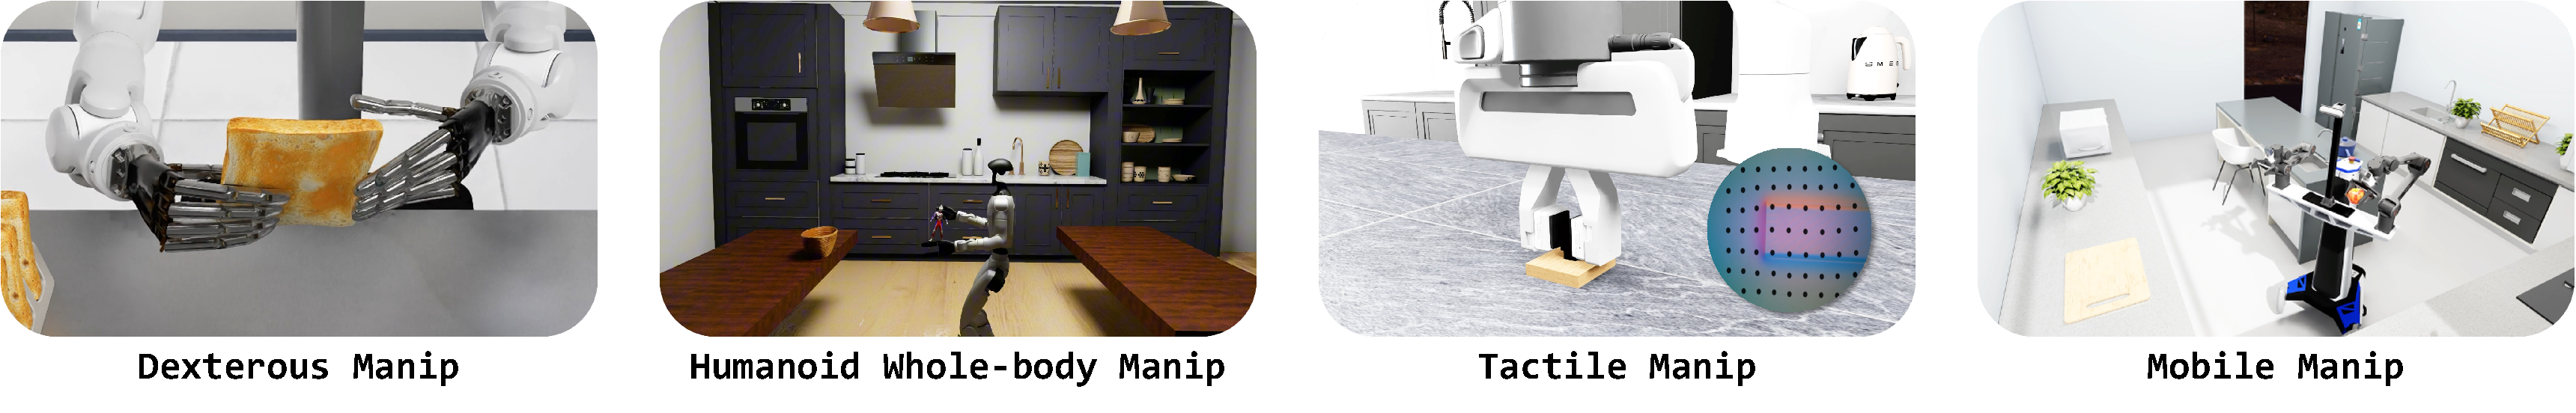
\includegraphics[width=1.0\textwidth]{assets/Figure/future.pdf}
    \caption{\textbf{Future extensions of RoboDojo.} RoboDojo will be continuously expanded to broader manipulation scenarios and embodiments, including dexterous hand manipulation, humanoid whole-body manipulation, tactile manipulation, and mobile manipulation.}

    \label{fig:future_work}
\end{figure}

RoboDojo is designed as an extensible benchmarking platform rather than a fixed task collection. In future releases, we will continuously expand RoboDojo toward broader scenarios, embodiments, and evaluation settings. As shown in Figure~\ref{fig:future_work}, we plan to introduce larger-scale benchmarks for dexterous hand manipulation, humanoid whole-body manipulation, tactile manipulation, and mobile manipulation. For each direction, RoboDojo will support multiple robot embodiments to improve accessibility and enable fair comparison across different hardware platforms. By progressively extending the task suite, embodiment coverage, and sensing modalities, RoboDojo aims to evolve into a general-purpose evaluation platform for embodied manipulation.